\subsubsection{State Charts}
In this section are illustrated the state charts of classes Tournament and Battle, to show the different states of these classes, and all possible transitions.\\

\textbf{Tournament State Chart:}
\begin{figure}[h]
    \centering
    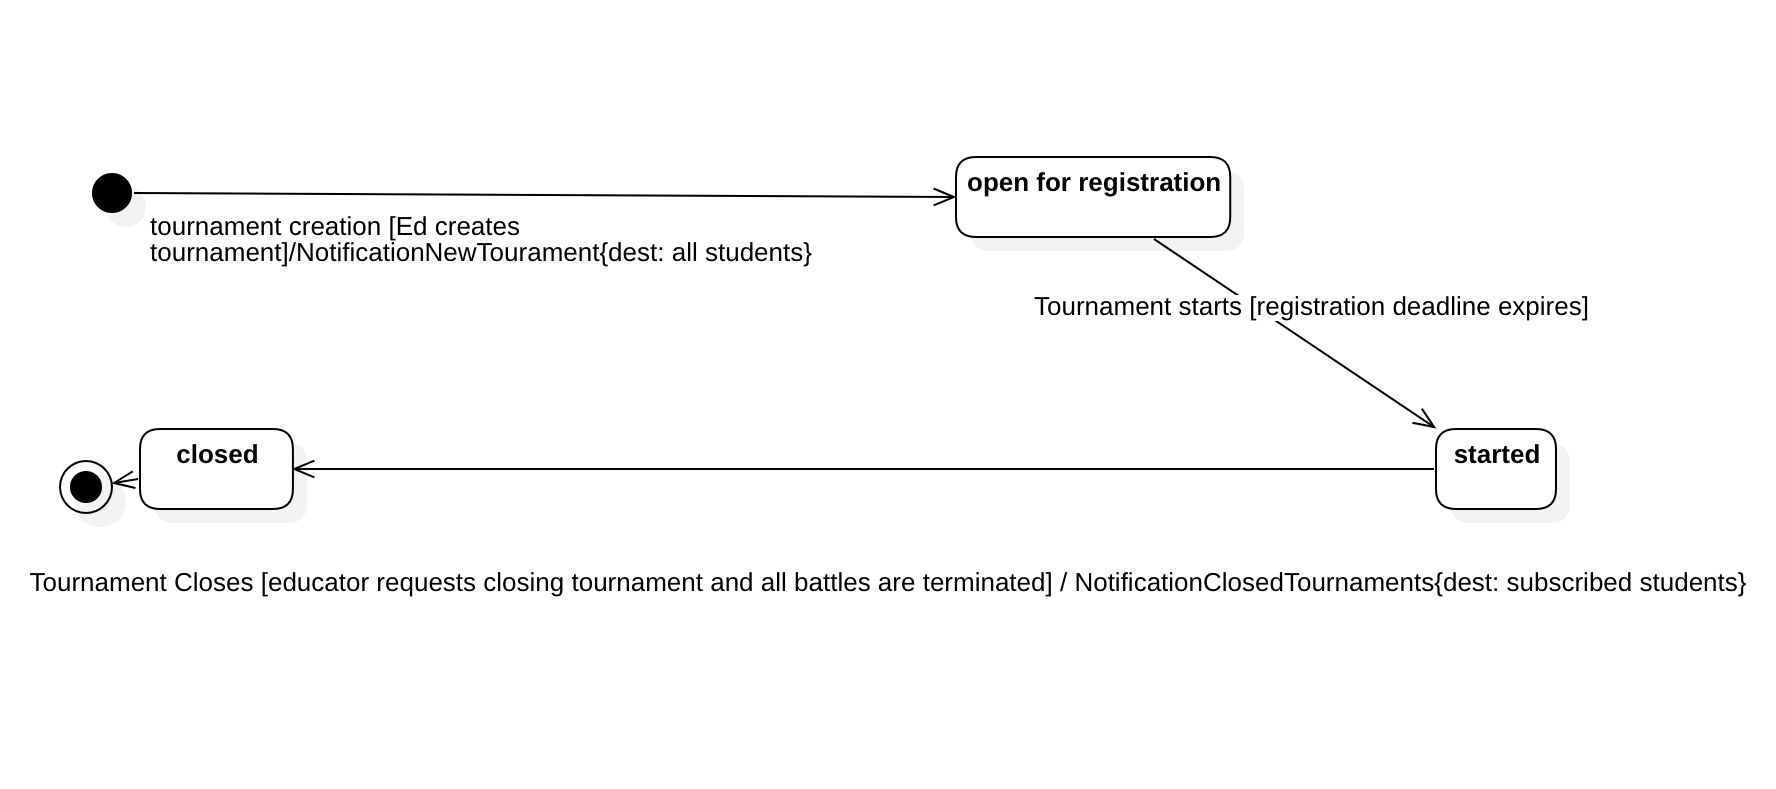
\includegraphics[width=1\textwidth]{RASD/2Overall_Description/res/st1.png}
\end{figure}

After an educator has created a tournament all the students can subscribe to it, this is the \textbf{Open for registration} state. After the registration deadline the tournament starts, student can't enroll anymore and edcucators can create battles, this is the \textbf{Started} state. When the educator that created the tournament decides it's time to close it, he can do so if there aren't ongoing battles, if he succeeds the tournament is closed (state \textbf{closed}).\\
\\
\clearpage
\textbf{Battle State Chart:}
\begin{figure}[h]
    \centering
    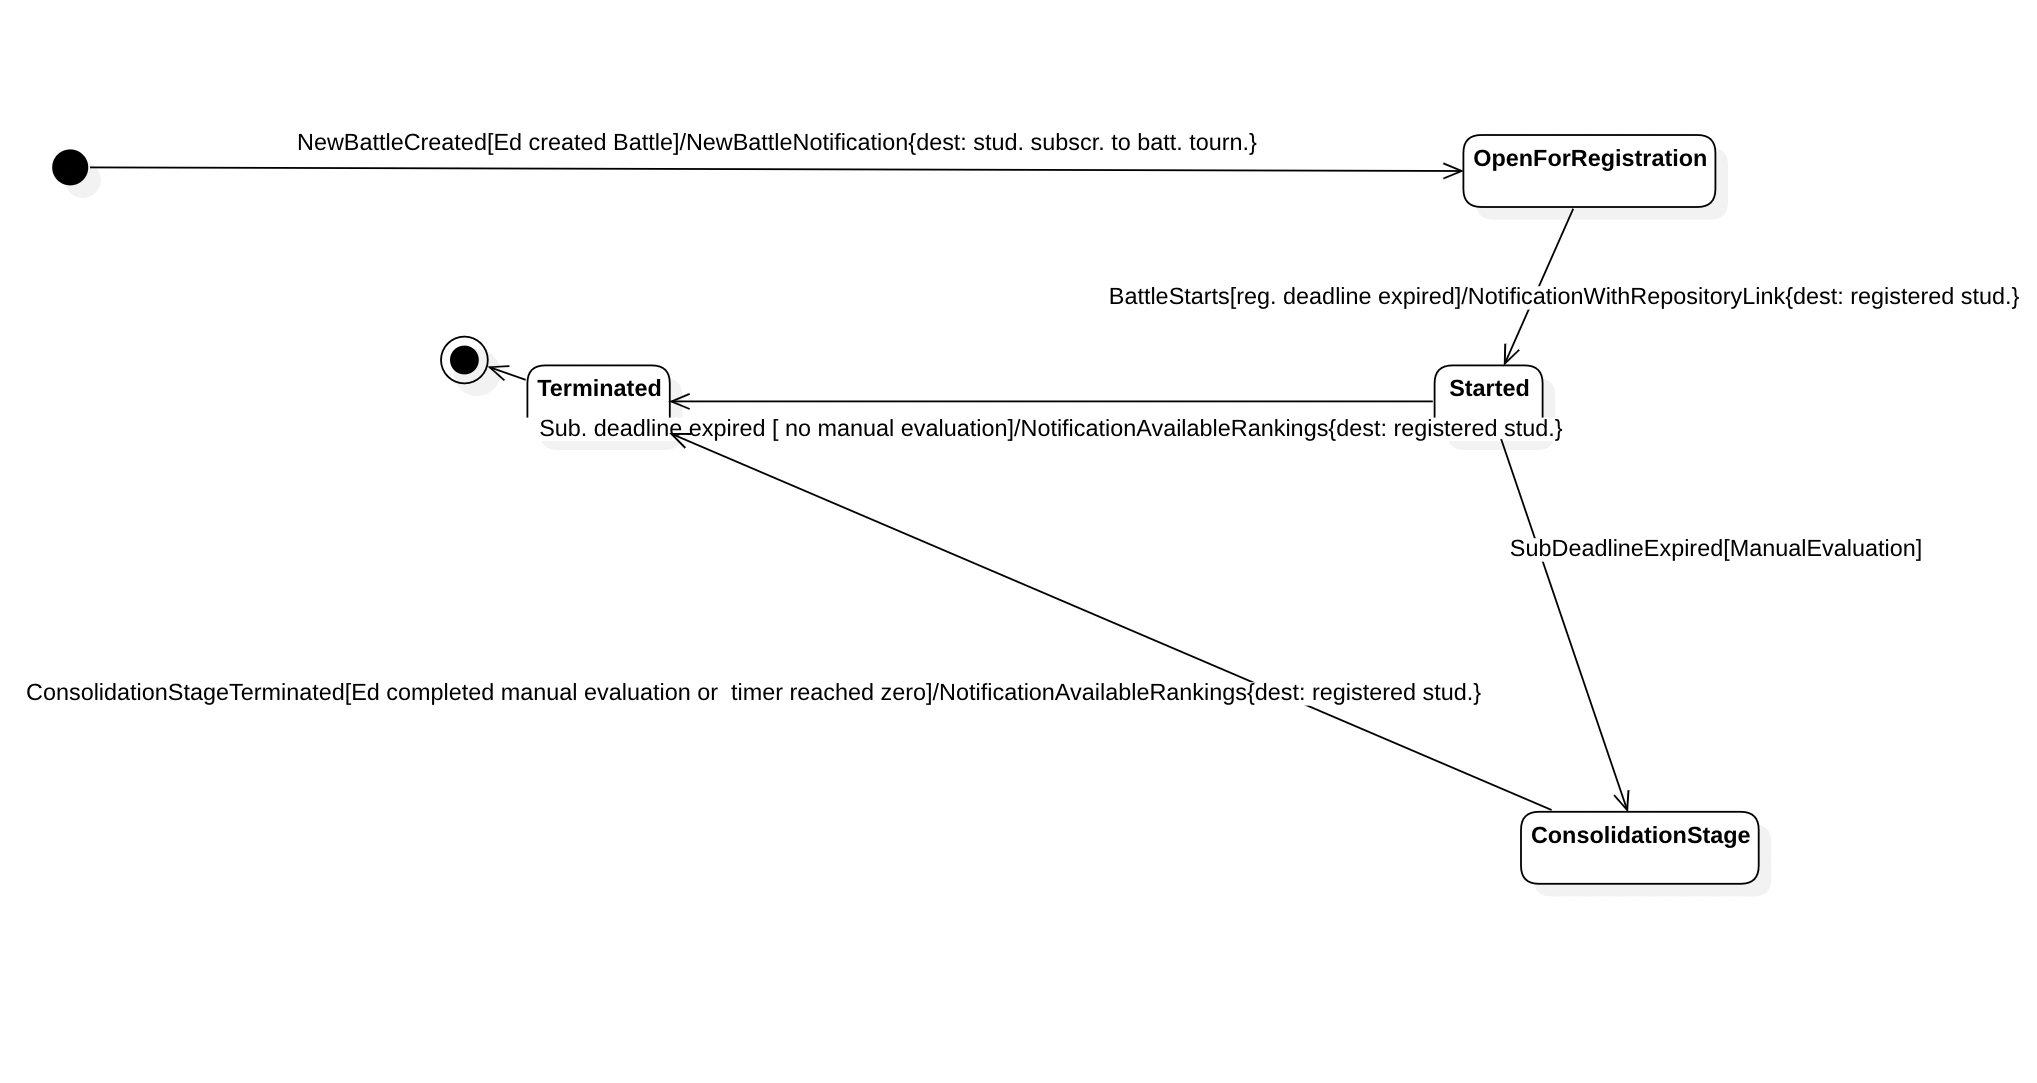
\includegraphics[width=1\textwidth]{RASD/2Overall_Description/res/stateChartBattle.png}
\end{figure}

After a battle is created students can enroll (\textbf{Open for registration} state). After the registration deadline students can't enroll anymore and a link to the battle repository is sent to all the registered students, (\textbf{Started} state). After the submission deadline, if the educator who created the battle has included a manual evaluation the Battle goes in a \textbf{Consolidation Stage} state. During the consolidation stage the educator assigns a score to each team last updated solution. The Battle goes from the consolidation stage state to \textbf{Terminated} state when the educator has finished grading all solutions, or when too much time has passed since the consolidation stage has started (fixed at 30 days). If no manual evaluation is expected, when the submission deadline expires the battle goes from the state \textbf{Started} to state \textbf{Terminated}.
